\documentclass{article}
\usepackage{amsmath}
\usepackage{amssymb}
\usepackage{amsthm}
\usepackage{MnSymbol}
\usepackage{xcolor}
\usepackage{parskip}
\usepackage{tikz}
\usepackage{bbm}
\usepackage{hyperref}
\usetikzlibrary{trees}
\usetikzlibrary{graphs}


\theoremstyle{definition}
\newtheorem{definition}{Definition}
\newtheorem{theorem}{Theorem}


\newcommand{\abs}[1]{\left| #1 \right|}


\title{lecture}
\date{\today}
\begin{document}
\maketitle


\section{HC}
\begin{equation}
    \max \sum_{ij\in E}^{} w_{ij}\sum_{k\neq ij}^{}\left( \mathbbm 1\{\text{k was the first ot be separated among ijk}\} \right)
\end{equation}

note the second sum is equal to \(n-\abs{T_{ij}}\) \label{1}

note on max cut:
random is at least 1/2 the optimal max cut


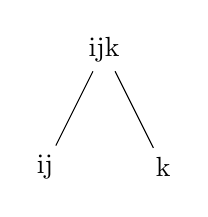
\begin{tikzpicture}
    \node{ijk}
    child{node{ij}}
    child{node{k}};
\end{tikzpicture}

this tree would contribute in the sum in the \ref{1}

a random HC gives 
\begin{equation}\label{2}
    \frac{1}{3}\sum_{ij\in E}^{}w_{ij}\left( n-1 \right)
\end{equation}

consider a \emph{matching} graph. 

\begin{tikzpicture}
    \graph{a -> b; c -> d;};
\end{tikzpicture}

where the arrows represent nonzero weights. 

the graph that is optimal and hits the bound given in \ref{2}

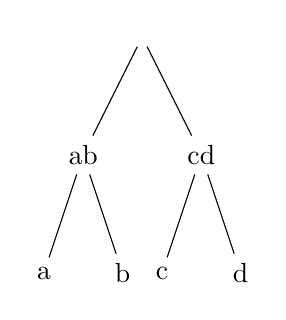
\begin{tikzpicture}[level 1/.style={sibling distance=15mm},
         level 2/.style={sibling distance=10mm}]
    \node{}
    child{node{ab} child{node{a}} child {node{b}}}
    child{node{cd} child{node{c}} child {node{d}}};
\end{tikzpicture}

for notatoon:
\begin{equation}
    P[ij\vert k]
\end{equation}

is defined as the probability of k being first separated from i,j

for 3 unit vectors combinations of ijk, \(\theta_ijk\), draw a random hyperplane again, if verticies are divided by the hyperplane, then they will be set into different branches of the tree.

if we assign the vectors for ijk randomly then do the hyperplane guess, we find the probability that ij are seperated before k to be

\begin{equation}
    P[ij\vert k] = \frac{\theta_{ik} + \theta_{jk} + \theta{ij}}{2\pi}
\end{equation}

for \begin{equation}
    \begin{split}
        P[ij\vert k]=&x\\
        P[jk\vert i]=&z\\
        P[ki\vert j]=&y\\
    \end{split}
\end{equation}

we see that
\begin{equation}
    x+z = P[i\vert k] = \frac{\theta_{ij}}{\pi}
\end{equation}

the sdp we are trying to maximize is 
\begin{equation}
    \sum_{ij\in E}^{}\sum_{t=1}^{n}w_{ij}\left( 1-x_{ij}^t \right)
\end{equation}

where \(t\) is each level in the graph

for the sdp version, we set 
\begin{equation}
    x_{ij}^t = \frac{1}{2}\abs{v_i^t-v_j^t}^2_2
\end{equation}













\end{document}